\documentclass[border=10pt]{standalone}
\usepackage{pgfplots}
\pgfplotsset{compat=1.17}
\begin{document}
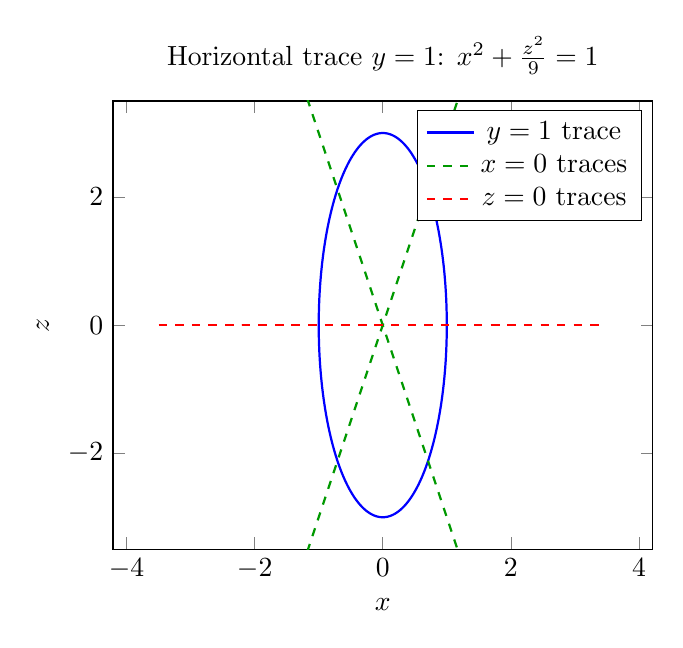
\begin{tikzpicture}
\begin{axis}[
    xlabel=$x$,
    ylabel=$z$,
    title={Horizontal trace $y=1$: $x^2+\frac{z^2}{9}=1$},
    xmin=-3.5, xmax=3.5,
    ymin=-3.5, ymax=3.5,
    axis equal,
    samples=200,
]
\addplot[blue,thick,domain=0:360] ({cos(x)},{3*sin(x)});
\addplot[green!60!black,dashed,thick,domain=-2:2] {3*x};
\addplot[green!60!black,dashed,thick,domain=-2:2] {-3*x};
\addplot[red,dashed,thick,domain=-3.5:3.5] {0};
\legend{$y=1$ trace, $x=0$ traces, , $z=0$ traces}
\end{axis}
\end{tikzpicture}
\end{document}
